
\chapter*{Solutions to Set \#5}
\addcontentsline{toc}{chapter}{Solutions to Set \#5}
\markboth{Solutions to Set \#5}{Solutions to Set \#5}
\label{set4sols}

\begin{sol}{prob:52}\index{$\Z_p$, ring of $p$-adic integers!introduction and basic properties} We check that $\Z_p$ contains the multiplicative identity $1 = (1\bmod{p}, 1\bmod{p^2}, 1\bmod{p^3}, \dots)$ of the ambient ring $\prod_{k=1}^{\infty} \Z/p^k$ and that $\Z_p$ is closed under subtraction and multiplication. The first requirement is clear. To prove the second and third, suppose $x, y \in \Z_{p}$. Write $x = (a_1\bmod{p}, a_2\bmod{p^2},\dots)$ and $y =  (b_1\bmod{p}, b_2\bmod{p^2},\dots)$, where $a_k \equiv a_{k+1} \pmod{p^k}$ and $b_k \equiv b_{k+1}\pmod{p^k}$
for all $k=1,2,3,\dots$. Then $a_k - b_k \equiv a_{k+1} - b_{k+1} \pmod{p^k}$ and $a_k b_k \equiv a_{k+1} b_{k+1} \pmod{p^k}$, for all $k=1,2,3,\dots$, These congruences imply that $x-y =(a_1-b_1\bmod{p},a_2-b_2\bmod{p^2}, \dots)$ and $xy = (a_1 b_1\bmod{p}, a_2 b_2\bmod{p^2}, \dots)$ also belong to $\Z_p$, as desired.
\end{sol}

\begin{sol}{prob:53} Suppose $x = (a_1\bmod{p},a_2\bmod{p^2}, \dots)$ and $y = (b_1\bmod{p}, b_2\bmod{p^2}, \dots)$ are nonzero elements of $\Z_p$. Since $x\ne 0$, there is an $i$ for which $p^i \nmid a_i$. Similarly, there is a $j$ for which $p^j \nmid b_j$. We will prove $xy\ne 0$ by showing that the mod $p^{i+j}$ component of $xy$ is nonzero, i.e., that $p^{i+j} \nmid a_{i+j} b_{i+j}$. 

The compatibility condition in the definition of $\Z_p$ assures us that $a_{i+j} \equiv a_i \not \equiv 0 \pmod{p^i}$. Similarly, $b_{i+j} \equiv b_j \not\equiv 0 \pmod{p^j}$. Therefore,
\[ v_p(a_{i+j} b_{i+j}) = v_p(a_{i+j}) + v_p(b_{i+j}) < i+j,\]
and $p^{i+j} \nmid a_{i+j} b_{i+j}$.
\end{sol}

\begin{sol}{prob:54} For each $n \in \Z^{+}$, the element $n\cdot 1$ of $\Z_p$ has a nonzero mod $p^k$ component whenever $p^k > n$. In particular, $n\cdot 1\ne 0$. Thus, $\Z_p$ has characteristic $0$, so that we can (and henceforth will!) view $\Z$ as a subring of $\Z_p$, identifying each integer $n$ with $n\cdot 1 = (n\bmod{p}, n\bmod{p^2}, n\bmod{p^3},\dots)$.

The rest of the problem asks (essentially) for a description of $\Q\cap \Z_p$. It may not be clear that this task even makes sense: To take this intersection, both $\Q$ and $\Z_p$ have to be viewed as sitting inside a common superset. What is that set? 

Fortunately, this question has an easy answer: Both $\Q$ and $\Z_p$ are contained in the fraction field of $\Z_p$. Taking this interpretation, if $a, b \in \Z$ with $b$ nonzero, $\frac{a}{b} \in \Q\cap \Z_p$ precisely when there is a $y \in \Z_p$ with $by=a$. When does this happen?

We can assume, without loss of generality, that $\gcd(a,b)=1$. If $p\mid b$, there is no hope of finding a $y$ with $by=a$: The mod $p$ component of $by$ is $0$ for every $y\in \Z_p$, while the mod $p$ component of $a$ is nonzero (remember that $\gcd(a,b)=1$, so that $p$ cannot divide $a$). Suppose instead that $p\nmid b$. In this case, we can choose integers $B_k$ with $b B_k \equiv 1\pmod{p^k}$, for $k=1,2,3,\dots$. Observing that $bB_{k+1}\equiv 1\pmod{p^{k+1}}$, we find that 
\[ bB_{k+1} \equiv 1 \equiv b B_k \pmod{p^k},\quad\text{and thus}\quad  B_{k+1} \equiv B_k \pmod{p^k}. \] Therefore $y_0 := (B_1\bmod{p}, B_2\bmod{p^2}, B_3\bmod{p^3},\dots) \in \Z_p$. Furthermore, $by_0 = (bB_1 \bmod{p}, bB_2\bmod{p^2}, \dots) = (1\bmod{p}, 1\bmod{p^2},\dots) = 1$, so that $y=ay_0$ satisfies $by=a$.

We conclude that $\Q\cap\Z_{p}$ is the set of rational numbers whose denominators, in lowest terms, are not multiples of $p$. This is precisely our faithful and familiar companion $\Z_{(p)}$. (Incidentally, this explains the term \textsf{$p$-integral} for elements of $\Z_{(p)}$; the $p$-integral rationals are the rational numbers that are also $p$-adic integers.)\index{$\Z_{(p)}$, ring of $p$-integral rationals}

As for the final question: Yes, $(4\bmod{5}, 34\bmod{5^2}, 334\bmod{5^3},\dots) \in \Q\cap \Z_5$. In fact, $3\cdot (4\bmod{5}, 34\bmod{5^2}, 334\bmod{5^3},\dots) = (12\bmod{5}, 102\bmod{5^2}, 1002\bmod{5^3}, \dots) = (2\bmod{5}, 2\bmod{5^2}, 2\bmod{5^3},\dots) =2$. 
\end{sol}

\begin{sol}{prob:55} Let $u=(a_1\bmod{p}, ,a_2\bmod{p}, \dots) \in \Z_p$. If $u \in \Z_p^{\times}$ with inverse $v = (b_1\bmod{p}, b_2\bmod{p^2}, \dots)$, then $uv = 1 = (1\bmod{p}, 1\bmod{p^2},\dots)$. Comparing mod $p$ components, $a_1 b_1\equiv 1\pmod{p}$. Thus, $a_1$ is invertible mod $p$, which implies that $p\nmid a_1$. 

Conversely, suppose that $p\nmid a_1$. Since each $a_k \equiv a_{k-1} \equiv \dots \equiv a_1\pmod{p}$, all of the $a_k$ are coprime to $p$. Choose integers $b_k$ with $a_k b_k \equiv 1\pmod{p^{k}}$, for $k=1,2,3,\dots$. Working modulo $p^{k+1}$,
\[ a_{k+1} b_{k+1} \equiv 1 \equiv a_k b_k \equiv a_{k+1} b_k, \]
so that $b_{k+1} \equiv b_k\pmod{p^k}$. Hence, $v:= (b_1\bmod{p}, b_2\bmod{p^2},\dots) \in \Z_p$. It is now straightforward to check that $uv=1$, so that $u \in \Z_{p}^{\times}$ (with $v =u^{-1}$). 

It remains to prove that $p\mid a_1$ (in $\Z$) $\Longleftrightarrow$ $p\mid u$ (in $\Z_p$). Suppose $p\mid u$ and write $u=pv$, where $v=(v_1\bmod{p}, v_2\bmod{p^2},\dots) \in \Z_p$. Then $a_1\equiv pv_1 \equiv 0\pmod{p}$, and $p\mid a_1$. 

Conversely, suppose $p\mid a_1$. Since each $a_k \equiv a_1\pmod{p}$, $p$ divides every $a_k$. Put $v_k = a_{k+1}/p$ for $k=1,2,3,\dots$. Dividing the congruence $a_{k+2}\equiv a_{k+1}\pmod{p^{k+1}}$ through by $p$ gives $v_{k+1}\equiv v_k\pmod{p^k}$, and so $v:=(v_1\bmod{p},  v_2\bmod{p^2}, \dots) \in \Z_p$. Moreover,
\[ pv = (a_2\bmod{p}, a_3\bmod{p^2}, \dots) = (a_1\bmod{p}, a_2\bmod{p^2}, \dots) = u.\]
(We use here that $a_{k+1}\equiv a_k\pmod{p^k}$ for each $k$.) Thus, $p\mid u$.
\end{sol}

\begin{sol}{prob:56} Let $x = (a_1\bmod{p}, a_2\bmod{p^2}, \dots)$ be a nonzero element of $\Z_p$ and choose the nonnegative integer $v$ minimally with $a_{v+1}\not\equiv 0\pmod{p^{v+1}}$. 
%If $v=0$, then $x$ is a unit in $\Z_p$, and $x = p^{0} x$ is an expression of the desired form. Now suppose that $v > 0$. 
For each integer $j > v$, 
\[ a_j \equiv a_{j-1} \equiv \dots \equiv a_{v+1} \equiv 0 \pmod{p^v}. \] 
(Consider two cases, $v=0$ or $v>0$.)  So  $b_k := p^{-v} a_{v+k} \in \Z$ for each $k=1,2,3,\dots$. The congruences $a_{v+k+1}\equiv a_{v+k} \pmod{p^{v+k}}$ imply that $b_{k+1}\equiv b_k\pmod{p^{k}}$. Therefore, $u:= (b_1\bmod{p}, b_2\bmod{p^2},\dots) \in \Z_{p}$. 

By the choice of $v$, we have that $p\nmid \frac{a_{v+1}}{p^v} = b_1$. Thus, $u \in \Z_{p}^\times$ (Exercise \ref{prob:55}). Furthermore,
\begin{align*} p^v u &= (0\bmod{p},\dots,0\bmod{p^v}, a_{2v+1}\bmod{p^{v+1}}, a_{2v+2}\bmod{p^{v+2}},\dots)\\
&= (0\bmod{p},\dots,0\bmod{p^v}, a_{v+1}\bmod{p^{v+1}}, a_{v+2}\bmod{p^{v+2}},\dots) = x.\end{align*} (Here we use that $a_{2v+i} \equiv a_{2v+i-1} \equiv \dots \equiv a_{v+i} \pmod{p^{v+i}}$.) So we have produced a representation $x=p^v u$ with $u \in \Z_{p}^\times$.

To prove uniqueness, suppose $x = p^{v} u = p^{v'} u'$ with $v, v'$ nonnegative integers and $u, u' \in \Z_{(p)}^{\times}$. Assume $v\le v'$. Canceling $p^{v}$ from both sides, $u = p^{v'-v} u'$. Since $u \in \Z_p^{\times}$, to avoid a contradiction with Exercise \ref{prob:55} we must have $v'-v=0$, i.e., $v=v'$. Then $p^v u = p^v u'$, leading to $u=u'$.
\end{sol}

\begin{sol}{prob:57} For each nonzero $x \in \Z_p$, define $v_p(x)$ as the integer $v$ appearing in the representation of $x$ described in Problem \ref{prob:56}. Then proceed as in the solution to Problem \ref{prob:39}. 
\end{sol}


\begin{sol}{prob:58} We preface the solution with some philosophical comments. With the definition we have given of $\Z_p$, there is an obvious \emph{informal} way to reduce $x$ modulo powers of $p$: Write $x=(a_1\bmod{p}, a_2\bmod{p^2}, \dots)$ and reduce mod $p^n$ by extracting the $n$th component, i.e., singling out $a_n\bmod{p^n}$. This defines the reduction of $x$ mod $p^n$ as an element of $\Z/p^n$. Since $\Z_p$ is a ring, there is also a \emph{canonical} way to reduce $x$ modulo $p^n$: Take the image of $x$ in $\Z_p/p^n\Z_p$. It would be reassuring if these two ways of reducing mod $p^n$ were somehow the same. As we will see shortly, this turns out to be the case! The isomorphism between $\Z/p^n$ and $\Z_p/p^n\Z_p$ induced by the inclusion $\Z\hookrightarrow \Z_p$  matches up $a_n\bmod{p^n}$ and $x\bmod{p^n\Z_p}$. Equivalently: $x\bmod{p^n\Z_p} = a_n\bmod{p^n\Z_p}$.

\epigraph{There is no justice in Heaven or Earth, but there is certainly justice in MATHEMATICS!}{Paul Erd\H{o}s}

We proceed to the proof proper. Let $\phi$ denote the homomorphism from $\Z$ to $\Z_p/p^n\Z_p$ induced by the inclusion $\Z\hookrightarrow \Z_p$. We start by computing the kernel of $\phi$. For $x \in \Z$,
\[ x \in \ker(\phi) \Longleftrightarrow
x \in p^n\Z_{p} \Longleftrightarrow x/p^n \in \Z_{p}\cap \Q \Longleftrightarrow x/p^n \in \Z_{(p)} \Longleftrightarrow x \in p^n\Z.
\]
(Here we have recalled that $\Q\cap \Z_{p} = \Z_{(p)}$.) So $\ker(\phi) = p^n\Z$, and $\phi$ induces an embedding $\tilde{\phi}\colon \Z/p^n \hookrightarrow \Z_p/p^n\Z_p$.

Next we show that $\phi$, and hence also $\tilde{\phi}$, is surjective.  Let $x = (a_1\bmod{p},a_2\bmod{p^2},\dots) \in \Z_{p}$. The mod $p^j$-component of $a_n-x$ is $a_n - a_j \bmod{p^j}$, which vanishes for all $j\le n$ (by the compatibility condition in the definition of $\Z_p$). So by our solution to Problem \ref{prob:56}, either $a_n-x=0$ or $a_n-x = p^k u$ for an integer $k \ge n$ and a unit $u \in \Z_p^{\times}$. In either case, $a_n-x \in p^n \Z_p$, so that $\phi(a_n) = a_n\bmod{p^n\Z_p} = x\bmod{p^n\Z_p}$. This proves $\phi$ is surjective, and so $\tilde{\phi}$ is an isomorphism. 

The isomorphism $\tilde{\phi}$ carries $a_n\bmod{p^n}$ to $\phi(a_n) =x\bmod{p^n\Z_{p}}$, as we promised in our initial remarks.
\end{sol}

\begin{sol}{prob:59}\index{$\Z_g$, ring of $g$-adic integers!decomposition as $\prod_{p\mid g}\Z_p$} Keeping in mind the Chinese Remainder Theorem, it is straightforward to check that $\Z_{g} \cong \prod_{p\mid g} \Z_{p^{v_p(g)}}$, via the map sending
\begin{multline*} (a_1\bmod{g}, a_2\bmod{g^2}, a_3\bmod{g^3},\dots) \\ \mapsto ((a_1\bmod{p^{v_p(g)}}, a_2\bmod{p^{2v_p(g)}}, a_3\bmod{p^{3v_p(g)}}, \dots))_{p\mid g}. \end{multline*} 
``Straightforward'' means that the tedium of writing out the proof outweighs the enlightenment gained from doing so. (Please walk through the argument in your head and decide if you agree!)

To complete the problem, it suffices to show that if $p$ is prime and $v \in \Z^{+}$, then $\Z_{p^v} \cong \Z_p$. Here we can map $(b_1\bmod{p^v}, b_2\bmod{p^{2v}}, b_3\bmod{p^{3v}}, \dots)$ to $(b_1\bmod{p},\dots, b_1\bmod{p^v},b_2\bmod{p^{v+1}},\dots,b_2\bmod{p^{2v}}, \dots)$, each $b_i$ repeated $v$ times. (Again, that this work is ``straightforward.'' Verify!)
\end{sol}



\begin{sol}{prob:60} The outer, red disc represents the entirety of $\Z_3$. The salmon-colored discs partition $\Z_3$ into three parts, based on  the mod $3$ component. Once the mod $3$ component is fixed, there are $3$ possibilities for the mod $3^2$ component, depicted by the green discs. Finally, having fixed the mod $3^2$ component, there are three possibilities for the mod $3^3$ component, illustrated by the purple discs. In theory this partitioning process could continue indefinitely, but at some point our eyes would ask for a break!

\begin{sol}{ex:dali} Who am I to tell you how to appreciate art?
\end{sol}

\begin{rmk} For further discussions around visualizing $\Z_p$, see \cite{cuoco91}, \cite{holly}, \cite[Chapter 2]{katok}, and \cite[Chapter 1, \S2]{robert}. 
\end{rmk}
\end{sol}

\begin{sol}{prob:61}  Let $f$ be any function from $\Z^{+}$ to $\Z_p$. We will show $f$ cannot be onto by adapting Cantor's famous \textsf{diagonal argument}. Choose a residue class $a_1\bmod{p}$ different from the mod $p$ component of $f(1)$. The class $a_1\bmod{p}$ lifts to $p$ residue class mod $p^2$; choose one, say $a_2\bmod{p^2}$, different from the mod $p^2$ component of  $f(2)$. This in turn lifts to $p$ classes mod $p^3$; choose one, say $a_3\bmod{p^3}$, different from the mod $p^3$ component of $f(3)$. Continue. At the end of the (very long) day, we find that $(a_1\bmod{p}, a_2\bmod{p^2}, a_3\bmod{p^3}, \dots)$ is an element of $\Z_{p}$ that cannot belong to the image of $f$, since it has a different mod $p^n$ component from $f(n)$ for each $n=1,2,3,\dots$. 
\end{sol}

\begin{challenge} Show that $\Z_p$ has the same cardinality as $\R$. A useful tool for this kind of proof is the \textsf{Cantor--Schr\"{o}der--Bernstein theorem}: \emph{If there are injections from $A$ to $B$ and from $B$ to $A$, then there is a bijection between $A$ and $B$}.\footnote{The author cannot resist outlining Cox's straightforward-to-verify proof of the Cantor--Schr\"{o}der--Bernstein result \cite{cox}. First, reduce to showing that if $f$ is an injection from a set $X$ to a subset $Y\subset X$, then there is a bijection between $X$ and $Y$. To tackle this new claim, put $S = \bigcup_{n=0}^{\infty} f^{(n)}(X\setminus Y) = (X\setminus Y) \cup f(X\setminus Y) \cup f(f(X\setminus Y)) \cup \dots$. Define $g\colon X\to Y$ by letting $g(x) = f(x)$ for $x\in S$ and $g(x) = x$ for $x\notin S$. Argue directly that $g$ is well-defined, injective, and surjective. }\index{Cantor--Schr\"{o}der--Bernstein theorem} 
\end{challenge}


\begin{sol}{prob:62}
\begin{figure}[t]
\centering
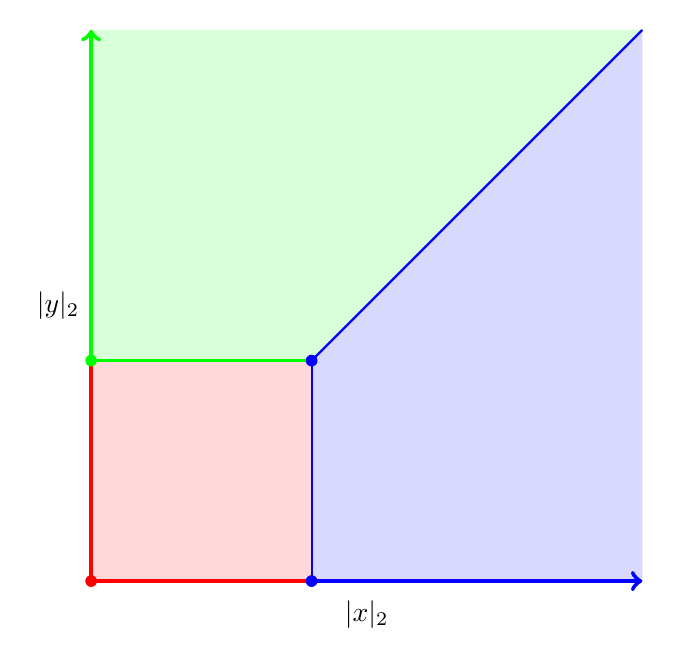
\begin{tikzpicture}[scale=0.7]
\node at (-0.6,5) {$|y|_2$};
\node at (5,-0.6) {$|x|_2$};
\filldraw [thick, fill=red!15] (0,0) rectangle (4,4);
\fill [fill=green!15, even odd rule] (0,4) -- (4,4) -- (10,10) -- (0,10) -- cycle;
\fill [fill=blue!15, even odd rule] (4,0) -- (10,0) -- (10,10) -- (4,4) -- cycle;
\draw[color=red, ultra thick] (0,0) -- (0,4);
\draw[color=red, ultra thick] (0,0) -- (4,0);
\draw[color=green, ultra thick,->] (0,4) -- (0,10);
\draw[color=blue, ultra thick,->] (4,0) -- (10,0);
\draw[color=red, thick] (0,0) -- (4,0);
\draw[color=red, thick] (0,0) -- (0,4);
\draw[color=green, thick] (0,4) -- (0,10);
\draw[color=blue, thick] (4,0) -- (10,0);
\draw[color=blue, thick] (4,4) -- (10,10);
\draw[color=green, thick] (0,4) -- (4,4);
\draw[color=blue,thick] (4,0) -- (4,4);
\node at (4,4) [color=blue,circle,fill,inner sep=1.5pt]{};
\node at (4,0) [color=blue,circle,fill,inner sep=1.5pt]{};
\node at (0,4) [color=green,circle,fill,inner sep=1.5pt]{};
\node at (0,0) [color=red,circle,fill,inner sep=1.5pt]{};
\end{tikzpicture}
\caption*{Coloring of $\Q^2$ in Problem \ref{prob:62}.}
\end{figure}
 Let $(x_r,y_r)$, $(x_b,y_b)$, and $(x_g, y_g)$ be the coordinates of the red, blue, and green vertices of $\Delta$. Then, by a formula  well-known to those who know it well,
\[ 2 \cdot \text{Area}(\Delta) = \pm \left|
\begin{matrix}
 x_b & y_b & 1 \\
x_g & y_g & 1 \\
x_r & y_r & 1
\end{matrix}
\right| = \pm (x_b y_g + x_r y_b + x_g y_r - x_g y_b - x_b y_r - x_r y_g).\]


We claim that $x_b y_g$ has $2$-adic absolute value strictly larger than the other five terms. By definition of the coloring, $|x_b y_g|_2 = |x_b|_{2} |y_g|_{2}\ge 1 \cdot 1 = 1$. Next, we observe that
\[ |x_r|_2 |y_b|_2 \le |x_r|_2 |x_b|_2 < |x_b|_2 \le |x_b|_2 |y_g|_2.  \]
If $y_r=0$, then $|x_g y_r|_2 = 0 < |x_b y_g|_2$; otherwise, 
\[  |x_g|_2 |y_r|_2 < |y_g|_2 |y_r|_2 < |y_g|_2 \le |x_b|_2 |y_g|_2. \]
If $y_b=0$, then $|x_g y_b|_2 = 0 < |x_b y_g|_2$; otherwise,
\[ |x_g|_2 |y_b|_{2} < |y_g|_{2} |y_b|_{2} \le |x_b|_2 |y_g|_{2}. \]
Next,
\[ |x_b|_2 |y_r|_{2} < |x_b|_2  \le |x_b|_2 |y_g|_{2}. \]
Finally, 
\[ |x_r|_2 |y_g|_2 < |y_g|_2 \le |x_b|_2 |y_g|_2.\]
Phew! 

Falling back on ``survival of the greatest,'' we conclude that $|2 \cdot\textrm{Area}(\Delta)|_{2} = |x_b y_g|_{2} \ge 1$, so that $|\textrm{Area}(\Delta)|_2 \ge |2|_2^{-1} > 1$.
\end{sol}


\begin{rmk} Here is a quick sketch of Monsky's proof.\index{Monsky's theorem} We can assume the square we are trying to dissect is $S = [0,1]\times [0,1] \subset \R^2$. 

Color $\Q^2$ as described in Problem \ref{prob:62}. A triangle with vertices from $\Q^2$ will be called a \textsf{rainbow triangle} if each vertex receives a different color. 

Suppose $S$ has been dissected into finitely many triangles. So that we can bring the coloring of $\Q^2$ into the picture, let's suppose that the vertices of all triangles appearing in the dissection have rational coordinates. 

Using a version of Sperner's lemma from combinatorial geometry, along with basic properties of our coloring, Monsky argues that the dissection must contain an \emph{odd} number of rainbow triangles. In particular, there is always at least one rainbow triangle $\Delta$ involved. As we showed above, $|\mathrm{Area}(\Delta)|_2 > 1$. So if we assume there are $n$ triangles involved in the dissection, each with the same area, then $|1/n|_2 > 1$; that is, $n$ is even. 

This is all well and good, but we are interested in arbitrary (real) dissections of $S$, not merely ``rational'' ones. Well, here is the astounding part: The same argument applies in the general case! At first glance this claim doesn't seem to make sense: Our initial coloring was defined in terms of $|\cdot|_2$, and $|\cdot|_2$ has domain $\Q$, not $\R$. It turns out, however, that it is possible to extend $|\cdot|_2$ to an absolute value on $\R$. (This is far from obvious!) With this extension in hand, everything else in the argument goes through with zero change.

A complete proof of Monsky's theorem can be found in \cite[Chapter 22]{AZ18}. The discussion in \cite{AZ18} sidesteps extending $|\cdot|_2$ to an absolute value on $\R$; the reader interested in seeing such an extension constructed can consult \S14 of  \cite{schikhof}.
\end{rmk}

\begin{challenge}[cf. Hales and Straus \cite{HS}] Let $K$ be an infinite field that can be endowed with a nontrivial, non-Archimedean absolute value. Show that it is possible to 3-color the affine plane $K^2$, using all three colors in an interesting way, so that every line receives points of at most two colors.  \textsf{In an interesting way} means that each color is assigned to three non-collinear points. (If we remove ``in an interesting way,'' this can be done for every infinite field. Can you see why?)
\end{challenge}

% \begin{challenge} Let $K$ be a field. It is always possible to 3-color the affine plane $K^2$, using all three colors, in such a way that every line receives points of at most two colors. For instance, color the origin red, then arbitrarily color each line through the origin (minus the origin itself) entirely blue or entirely green, making sure to use both of those colors at least once. 

% To keep the problem interesting, call a 3-coloring of $K^2$ \textsf{nontrivial} if each color is assigned to three non-collinear points. Show that if $K$ admits a nontrivial non-Archimedean absolute value, then $K^2$ admits a nontrivial 3-coloring where each line contains points of at most two colors. (Fields $K$ admitting nontrivial $3$-colorings of this kind are characterized in \cite{HS}.)
% \end{challenge}

\begin{challenge}[Hensel's definition of the $p$-adic integers]\index{$\Z_p$, ring of $p$-adic integers!Hensel's definition} Let $\phi\colon \Z[[T]] \to \prod_{k=1}^{\infty} \Z/p^k$ be the map sending $a_0 + a_1 T + a_2 T^2 + \dots$ to $(a_0 \bmod{p}, a_0 + a_1 p \bmod{p^2}, a_0 + a_1 p + a_2 p^2 \bmod{p^3}, \dots)$. Here the $k$th component of the output is  $a_0 + a_1 p + \dots + a_{k-1} p^{k-1}\bmod p^k$. 
\vspace{-0.12in}
\begin{enumerate} 
    \item[(a)] Check that $\phi$ is a ring homomorphism.
    \item[(b)] Show that $\phi(\Z[[T]]) = \Z_p$. 

{\scriptsize If you squint just right, 
you can see Hensel defining the $p$-adic integers in \cite{hensel13} as the quotient $\Z[[T]]/\ker(\phi)$. This claim must be taken \textsl{cum grano salis}; even the notion of a ``ring''  was still up in the air when \cite{hensel13} was written. Nevertheless, it gets at the essence of Hensel's description.}

\item[(c)] Show that $\ker(\phi) = (T-p)\Z[[T]]$. 
\end{enumerate}
\end{challenge}

\begin{rmk} 
% In addition to anachronistically importing modern concepts (e.g., homomorphisms and their kernels), this take on Hensel's definition disregards Hensel's constructivist requirement that the power series under consideration have coefficients that ``can be calculated as far as desired.''
It seems that neither the definition in \cite{hensel13}, nor Hensel's earlier descriptions in \cite{hensel04, hensel08} (similar but less refined), were viewed by Hensel's contemporaries as entirely rigorous. In his obituary \cite{hasse} for Hensel, Hasse describes the $p$-adic numbers as ``a genuine creation driven by intuition and imagination, which, initially, like every revolutionary idea, was thrown down bluntly and in raw form and which, similar to Leibniz's differential calculus, initially lacked a solid logical foundation.'' Apprehensions about the logical standing of $p$-adic numbers were dispelled only after Kürschák and Ostrowski's papers on valuation theory, which began to appear around the same time as \cite{hensel13}.
\end{rmk}


\let\oldaddcontentsline\addcontentsline
\renewcommand{\addcontentsline}[3]{}
\begin{thebibliography}{11}

\bibitem{AZ18} M. Aigner and {G.\,M}. Ziegler, \emph{Proofs from The Book},
sixth edition, Springer, Berlin, 2018.

\bibitem{cox} R.\,H. Cox, \emph{A proof of the {S}chroeder-{B}ernstein theorem}. Amer. Math. Monthly \textbf{75} (1968), 508.

\bibitem{cuoco91} {A.\,A.} Cuoco,
\emph{Visualizing the $p$-adic integers}. Amer. Math. Monthly \textbf{98} (1991), 355--36.

\bibitem{HS} {A.\,W.} Hales and {E.\,G.} Straus, \emph{Projective colorings}. Pacific J. Math. \textbf{99} (1982), 31--43. 

\bibitem{hasse} H. Hasse, \emph{Kurt Hensel zum Gedächtnis}. J. Reine Angew. Math. \textbf{187} (1949), 1--13.

\bibitem{hensel04} K. Hensel, \emph{Neue Grundlagen der Arithmetik}. J. Reine Angew. Math. \textbf{127} (1904), 51--84.

\bibitem{hensel08} \bysame, \emph{Theorie der algebraischen Zahlen}, {B.\,G.} Teubner, Leipzig and Berlin, 1908.  

\bibitem{hensel13} \bysame, \emph{Zahlentheorie}, {G.\,J.} Göschen, Berlin and Leipzig, 1913.  

\bibitem{holly} {J.\,E.} Holly, 
\emph{Pictures of ultrametric spaces, the $p$-adic numbers, and valued fields}. Amer. Math. Monthly \textbf{108} (2001), 721--728.

\bibitem{katok} S.~Katok, \emph{{$p$}-adic analysis compared with real}, Student Mathematical Library, vol.~37, American Mathematical Society, Providence, RI; Mathematics Advanced Study Semesters, University Park, PA, 2007. 

\bibitem{robert} {A.\,M.} Robert, \emph{A course in p-adic analysis}, Grad. Texts in Math., vol.~198, Springer-Verlag, New York, 2000.   

\bibitem{schikhof} {W.\,H.}~Schikhof, \emph{Ultrametric calculus:  An introduction to $p$-adic analysis}, Cambridge Studies in Advanced Mathematics, vol.~4, Cambridge University Press, Cambridge, 2006.
 \end{thebibliography}
\let\addcontentsline\oldaddcontentsline

